\documentclass[handout]{mcs}

\begin{document}

\microquiz{Feb. 22, afternoon}

%%%%%%%%%%%%%%%%%%%%%%%%%%%%%%%%%%%%%%%%%%%%%%%%%%%%%%%%%%%%%%%%%%%%%
% Problems start here
%%%%%%%%%%%%%%%%%%%%%%%%%%%%%%%%%%%%%%%%%%%%%%%%%%%%%%%%%%%%%%%%%%%%%

\begin{problem}
Consider the function shown in Fig. \ref{fig:img} 

\begin{figure}[h]

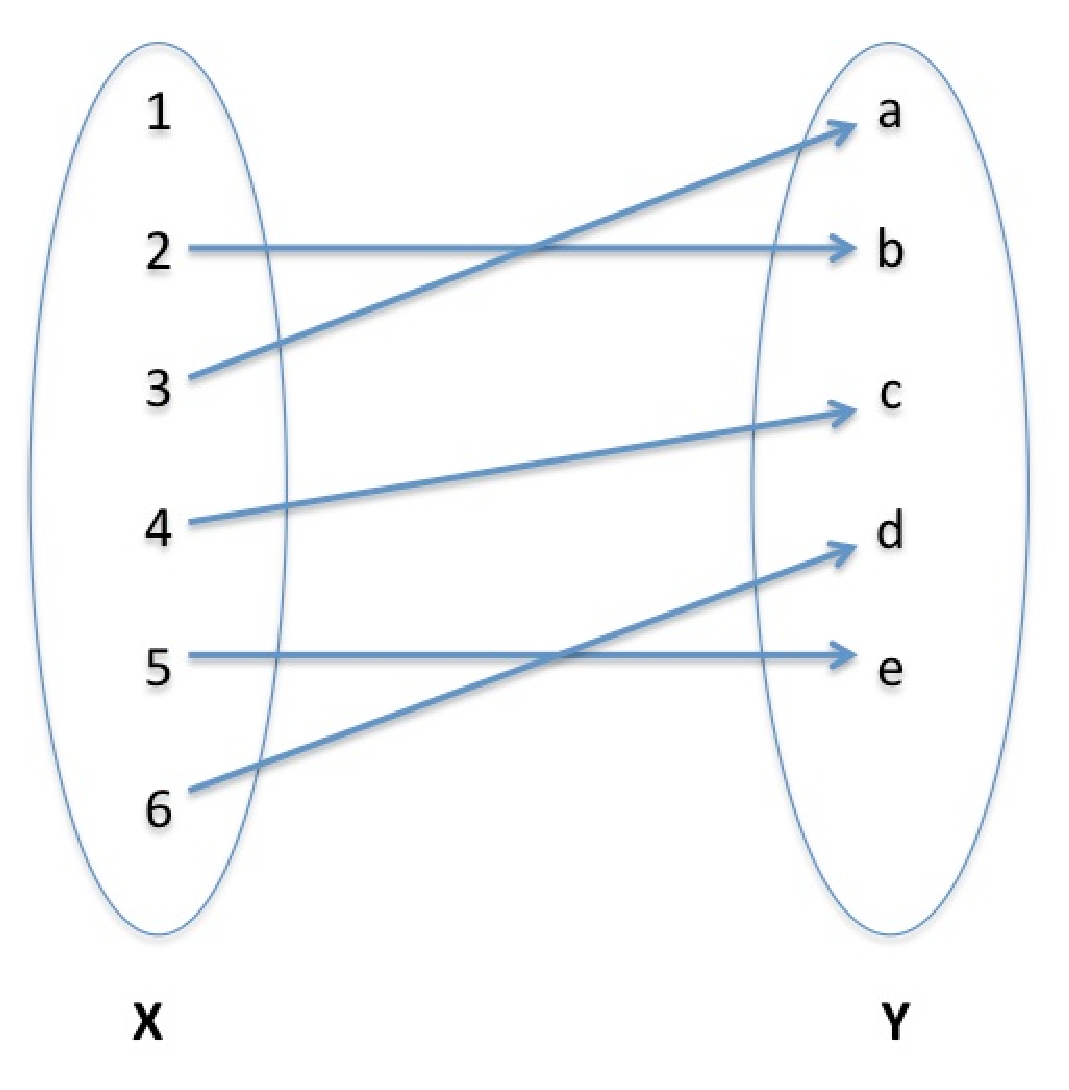
\includegraphics[height = 5in ]{image-inverseimage2}

\caption{Relation $R$.}
\label{fig:img}
\end{figure}

\bparts

\ppart What is the image of X? What is the inverse image of Y?

\ppart What is the image of the subset of X containing only even numbers? Only odd numbers?

\ppart What is the inverse image of the subset of Y containing only vowels? Only consonants?

\ppart Is the function (i) total? (ii) injective? (iii) bijective? (iv) surjective?

\end{problem}

%%%%%%%%%%%%%%%%%%%%%%%%%%%%%%%%%%%%%%%%%%%%%%%%%%%%%%%%%%%%%%%%%%%%%
% Problems end here
%%%%%%%%%%%%%%%%%%%%%%%%%%%%%%%%%%%%%%%%%%%%%%%%%%%%%%%%%%%%%%%%%%%%%
\end{document}
